
% !TEX program = pdflatex
\documentclass[aspectratio=169,10pt]{beamer}

% ----------------------
% Theme / look
% ----------------------
\usetheme{Madrid}
\usecolortheme{default}
\setbeamertemplate{navigation symbols}{}
\setbeamertemplate{footline}{}
\setbeamertemplate{caption}[numbered]
\usefonttheme{professionalfonts}

% ----------------------
% Packages
% ----------------------
\usepackage{amsmath, amssymb, bm, mathtools}
\usepackage{graphicx}
\usepackage{booktabs, tabularx, array}
\usepackage{siunitx}
\usepackage{tikz}
\usepackage{pgfplots}
\usepackage[american,siunitx]{circuitikz}
\pgfplotsset{compat=1.18}
\usetikzlibrary{arrows.meta, positioning, calc, shapes, patterns,
                 decorations.pathreplacing, fit}

\usepackage[most]{tcolorbox}
\usepackage{listings}
\usepackage{xcolor}

% ----------------------
% Graphics
% ----------------------
\graphicspath{{Figures/}}

% ----------------------
% Listings (MATLAB)
% ----------------------
\lstdefinelanguage{Matlab}{
  keywords={break,case,catch,continue,else,elseif,end,for,function,global,
            if,otherwise,persistent,return,switch,try,while},
  morekeywords={sdpvar,optimize,sdpsettings,quadprog,linprog,value,
                expm,ss,c2d,ode45,zeros,ones,size,disp,clear,clc,eye,
                diag,eig,ctrb,obsv,rank,fprintf},
  sensitive=true,
  morecomment=[l]\%,
  morestring=[m]'
}
\lstset{
  language=Matlab,
  basicstyle=\ttfamily\scriptsize,
  keywordstyle=\color{blue!70!black}\bfseries,
  commentstyle=\color{green!40!black},
  stringstyle=\color{orange!70!black},
  numbers=left,
  numberstyle=\tiny\color{gray!70},
  stepnumber=1,
  numbersep=6pt,
  tabsize=2,
  showstringspaces=false,
  breaklines=true,
  breakatwhitespace=false,
  frame=single,
  rulecolor=\color{gray!40}
}

% ----------------------
% Box styles
% ----------------------
\tcbset{
  beamer,
  enhanced,
  colback=white,
  colframe=blue!60!black,
  boxrule=0.6pt,
  arc=2pt,
  left=6pt,right=6pt,top=4pt,bottom=4pt
}
\newtcolorbox{defnbox}[1]{title=#1, colframe=blue!70!black, colback=blue!3}
\newtcolorbox{notebox}[1]{title=#1, colframe=teal!70!black, colback=teal!3}
\newtcolorbox{examplebox}[1]{title=#1, colframe=orange!80!black, colback=orange!3}
\newtcolorbox{alertbox}[1]{title=#1, colframe=red!75!black, colback=red!4}
\newtcolorbox{summarybox}[1]{title=#1, colframe=purple!70!black, colback=purple!4}

% ----------------------
% Convenience macros
% ----------------------
\newcommand{\R}{\mathbb{R}}
\newcommand{\T}{^\top}
\newcommand{\dd}{\,\mathrm{d}}
\newcommand{\Ccal}{\mathcal{C}}
\newcommand{\Ocal}{\mathcal{O}}

% ----------------------
% Metadata
% ----------------------
\title[State-Space, Controllability \& Observability]%
      {State-Space Representation,\\Controllability \& Observability}
\subtitle{MSc Model Predictive Control --- Chapters 3 \& 4}
\author{Dr ~\.{I}brahim K\"{u}\c{c}\"{u}kdemiral}
\institute{Glasgow Caledonian University}
\date{\today}

\begin{document}

% =============================================================
%  TITLE
% =============================================================
\begin{frame}
\titlepage
\end{frame}

% =============================================================
%  LEARNING OBJECTIVES
% =============================================================
\begin{frame}{Learning objectives}
After completing these slides you should be able to:
\begin{enumerate}
  \item Write continuous-time state-space models from physical first principles.
  \item Identify equilibrium points and linearise nonlinear systems using Jacobians.
  \item Discretise LTI systems exactly (ZOH / matrix exponential) and nonlinear systems approximately (Euler, RK4).
  \item Assess discrete-time stability via eigenvalue location and Lyapunov theory.
  \item Construct and evaluate the controllability matrix $\Ccal$ and observability matrix $\Ocal$.
  \item Apply the Kalman rank condition to determine whether a system can be controlled and/or observed.
  \item Understand why these structural properties are prerequisites for MPC and observer design.
\end{enumerate}
\end{frame}

% =============================================================
%  TABLE OF CONTENTS
% =============================================================
\begin{frame}{Outline}
\tableofcontents
\end{frame}

% #############################################################
%  PART I: STATE-SPACE REPRESENTATION  (Chapter 3)
% #############################################################

\part{State-Space Representation}

\section{Introduction to state-space models}

% =============================================================
\begin{frame}{A guiding thought}
\begin{quote}
\itshape
``The sciences do not try to explain, they hardly even try to interpret,
they mainly make models.  By a model is meant a mathematical construct
which, with the addition of certain verbal interpretations, describes
observed phenomena.''
\end{quote}
\hfill --- \textbf{John von Neumann}
\end{frame}

% =============================================================
\begin{frame}{Why this chapter matters for MPC}
The quality of any MPC controller depends directly on the quality of the
prediction model.  To predict future trajectories and optimise future
inputs, we need a mathematical representation that is:
\begin{itemize}
  \item accurate enough to capture the relevant dynamics,
  \item structured enough to analyse,
  \item efficient enough for real-time computation.
\end{itemize}

In practice:
\begin{itemize}
  \item physical systems are \textbf{continuous-time},
  \item many systems are \textbf{nonlinear},
  \item controllers are implemented \textbf{digitally},
  \item many standard MPC formulations rely on \textbf{linear discrete-time models}.
\end{itemize}

\begin{notebox}{Flow of ideas}
Physics $\rightarrow$ state-space model $\rightarrow$ equilibrium
$\rightarrow$ linearisation $\rightarrow$ discretisation
$\rightarrow$ MPC prediction model.
\end{notebox}
\end{frame}

% =============================================================
\begin{frame}{What is state-space, and why is it central to MPC?}
State-space modelling describes a dynamic system using a set of
\textbf{internal variables} called states.

\begin{defnbox}{Central principle}
If the state $x(t)$ is known at a given time, and the future inputs are
known, then the future behaviour of the system is fully determined.
\end{defnbox}

This is exactly the property required by MPC:
\begin{itemize}
  \item the controller measures or estimates the current state,
  \item predicts future states and outputs over a horizon,
  \item computes an optimal future input sequence.
\end{itemize}
\end{frame}

% =============================================================
\begin{frame}{General nonlinear continuous-time state-space model}
A general nonlinear continuous-time state-space model is
\[
\dot{x}(t)=f\!\big(x(t),u(t),t\big),
\qquad
y(t)=h\!\big(x(t),u(t),t\big).
\]

Here:
\begin{itemize}
  \item $x(t)\in\R^n$: state vector (internal variables),
  \item $u(t)\in\R^m$: input vector (control actions),
  \item $y(t)\in\R^p$: output vector (measurements),
  \item $f(\cdot)$: dynamics map ($n$ coupled first-order ODEs),
  \item $h(\cdot)$: output map.
\end{itemize}

\begin{notebox}{Interpretation}
This compact vector form is a structured way of writing $n$ coupled
first-order differential equations.
\end{notebox}
\end{frame}

% =============================================================
\begin{frame}{Expanded state and output equations}
\[
\underbrace{
\begin{bmatrix}
\dot{x}_1(t)\\
\dot{x}_2(t)\\
\vdots\\
\dot{x}_n(t)
\end{bmatrix}}_{\dot{x}(t)}
\!=\!
\underbrace{
\begin{bmatrix}
f_1(x_1,\dots,x_n,\,u_1,\dots,u_m,\,t)\\
f_2(x_1,\dots,x_n,\,u_1,\dots,u_m,\,t)\\
\vdots\\
f_n(x_1,\dots,x_n,\,u_1,\dots,u_m,\,t)
\end{bmatrix}}_{f(x(t),u(t),t)},
\qquad
\underbrace{
\begin{bmatrix}
y_1(t)\\
\vdots\\
y_p(t)
\end{bmatrix}}_{y(t)}
\!=\!
\underbrace{
\begin{bmatrix}
h_1(\cdot)\\
\vdots\\
h_p(\cdot)
\end{bmatrix}}_{h(x(t),u(t),t)}
\]

\begin{itemize}
  \item $x_i(t)$: the $i$-th state (e.g.\ position, voltage),
  \item $u_j(t)$: the $j$-th input (e.g.\ force, current),
  \item $f_i(\cdot)$: the $i$-th differential equation,
  \item $h_k(\cdot)$: the $k$-th output equation.
\end{itemize}
\end{frame}

% =============================================================
\begin{frame}{Linear Time-Invariant (LTI) state-space form}
For linear time-invariant systems the model simplifies to
\begin{align*}
\dot{x}(t) &= Ax(t)+Bu(t),\\
y(t) &= Cx(t)+Du(t).
\end{align*}

The matrices have clear roles:
\begin{center}
\renewcommand{\arraystretch}{1.25}
\begin{tabular}{cl}
\toprule
Matrix & Role \\ \midrule
$A\in\R^{n\times n}$ & Internal (autonomous) dynamics \\
$B\in\R^{n\times m}$ & Input-to-state coupling \\
$C\in\R^{p\times n}$ & State-to-output mapping \\
$D\in\R^{p\times m}$ & Direct feedthrough (often zero) \\
\bottomrule
\end{tabular}
\end{center}

\begin{notebox}{Why this matters in MPC}
LTI models lead naturally to efficient predictions and convex QP
optimisation problems.
\end{notebox}
\end{frame}

% =============================================================
\begin{frame}{Physical interpretation of states}
In practice, states usually correspond to variables associated with
\textbf{stored energy} or internal configuration:
\begin{itemize}
  \item \textbf{Electrical systems:} inductor currents, capacitor voltages
        (magnetic and electric energy).
  \item \textbf{Mechanical systems:} positions and velocities
        (potential and kinetic energy).
  \item \textbf{Process systems:} temperatures, pressures, concentrations
        (thermal / chemical potential).
\end{itemize}

\begin{notebox}{Important caveat}
We may also intentionally add non-physical states such as:
\begin{itemize}
  \item integral states (for offset-free tracking),
  \item disturbance estimates,
  \item bias states.
\end{itemize}
These are mathematical constructs but are treated identically in the framework.
\end{notebox}
\end{frame}

% =============================================================
\begin{frame}{Why state-space is so useful for MPC}
\begin{itemize}
  \item \textbf{Recursive prediction:}
        $x_{k+1}=A_d x_k + B_d u_k$ is iterated step by step.
  \item \textbf{Native MIMO description:}
        multiple inputs and outputs handled directly via matrix dimensions.
  \item \textbf{Direct constraint handling:}
        physical limits map to simple linear inequalities $Cx + Du \le b$.
  \item \textbf{Systematic discretisation:}
        continuous-time physics $\rightarrow$ discrete-time prediction equations.
\end{itemize}

\begin{alertbox}{Bottom line}
State-space is the modelling language that links physical intuition,
mathematical analysis, and predictive control design.
\end{alertbox}
\end{frame}

% =============================================================
\section{Modelling from physical laws}

% =============================================================
\begin{frame}{Example: simple pendulum --- physical setup}
\begin{columns}[T,totalwidth=\textwidth]
\begin{column}{0.40\textwidth}
\begin{center}
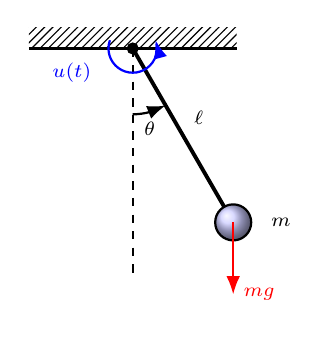
\begin{tikzpicture}[thick, >=Latex, scale=0.88]
  \fill [pattern = north east lines] (-1.5,0) rectangle (1.5,0.3);
  \draw (-1.5,0) -- (1.5,0);
  \filldraw [black] (0,0) circle (2pt);
  \draw [dashed] (0,0) -- (0,-3.3);
  \draw [line width=1.4pt] (0,0) -- (1.45,-2.51)
        node [midway, above right] {\scriptsize $\ell$};
  \shade [ball color=blue!20] (1.45,-2.51) circle (0.26);
  \draw (1.45,-2.51) circle (0.26) node [right=0.35cm] {\scriptsize $m$};
  \draw [->] (0,-0.95) arc (270:300:0.95)
        node [midway, below] {\scriptsize $\theta$};
  \draw [->, red] (1.45,-2.51) -- (1.45,-3.55)
        node [right] {\scriptsize $mg$};
  \draw [->, blue, domain=160:380] plot ({0.35*cos(\x)}, {0.35*sin(\x)});
  \node [blue, left] at (-0.45,-0.35) {\scriptsize $u(t)$};
\end{tikzpicture}
\end{center}
\end{column}
\begin{column}{0.58\textwidth}
Apply rotational Newton's law:
\[
\tau_{\text{net}} = I\ddot{\theta},\qquad I=m\ell^2.
\]

Torques acting on the pendulum:
\begin{itemize}
  \item control torque: $+u(t)$,
  \item gravity: $-mg\ell\sin\theta$,
  \item viscous damping: $-b\dot{\theta}$.
\end{itemize}

Hence
\[
m\ell^2 \ddot{\theta}=u(t)-mg\ell\sin\theta-b\dot{\theta},
\]
so
\[
\ddot{\theta}=
-\frac{g}{\ell}\sin\theta
-\frac{b}{m\ell^2}\dot{\theta}
+\frac{1}{m\ell^2}u(t).
\]
\end{column}
\end{columns}
\end{frame}

% =============================================================
\begin{frame}{Pendulum: nonlinear state-space form}
Choose the states
\[
x_1(t)=\theta(t),\qquad x_2(t)=\dot{\theta}(t).
\]

Then
\begin{align*}
\dot{x}_1 &= x_2,\\
\dot{x}_2 &= -\frac{g}{\ell}\sin(x_1)
              -\frac{b}{m\ell^2}x_2
              +\frac{1}{m\ell^2}u.
\end{align*}

In vector form:
\[
\dot{x}=
\begin{bmatrix}
x_2\\[4pt]
-\dfrac{g}{\ell}\sin(x_1)
-\dfrac{b}{m\ell^2}x_2
+\dfrac{1}{m\ell^2}u
\end{bmatrix},
\qquad
y=\begin{bmatrix}1 & 0\end{bmatrix}x = x_1.
\]

\begin{notebox}{Observation}
This is a \textbf{nonlinear} state-space model because of the
$\sin(x_1)$ term.
\end{notebox}
\end{frame}

% =============================================================
\begin{frame}{Pendulum: small-angle linearisation}
Near the downward equilibrium $\theta=0$, use
$\sin(\theta)\approx\theta$:
\begin{align*}
\dot{x}_1 &= x_2,\\
\dot{x}_2 &= -\frac{g}{\ell}x_1
              -\frac{b}{m\ell^2}x_2
              +\frac{1}{m\ell^2}u.
\end{align*}

Hence $\dot{x}=Ax+Bu$, with
\[
A=
\begin{bmatrix}
0 & 1\\[4pt]
-\dfrac{g}{\ell} & -\dfrac{b}{m\ell^2}
\end{bmatrix},
\qquad
B=
\begin{bmatrix}
0\\[4pt]
\dfrac{1}{m\ell^2}
\end{bmatrix},
\qquad
C=\begin{bmatrix}1 & 0\end{bmatrix},
\quad
D=0.
\]

This is the standard LTI quadruplet $(A,B,C,D)$, ready for discretisation and MPC design.
\end{frame}

% =============================================================
\begin{frame}{Example: RLC circuit --- circuit and states}
\begin{columns}[T,totalwidth=\textwidth]
\begin{column}{0.45\textwidth}
\begin{center}
\begin{circuitikz}[scale=0.68]
  \draw (2, 5) to[sinusoidal voltage source, l={$V_i$}] (2, 9);
  \draw (2, 9) to[american resistor, l={$R_1$}] (5, 9);
  \node[circ] at (5, 9){};
  \draw (5, 9) to[cute inductor, l={$L$}] (5, 5);
  \draw (5, 9) to[american resistor, l={$R_2$}] (8, 9);
  \node[circ] at (8, 9){};
  \draw (8, 9) to[capacitor, l={$C$}] (8, 5);
  \node[circ] at (5, 5){};
  \draw (8, 5) -- (5, 5) -- (2, 5);
  \node[ground] at (5, 5){};
  \draw[-Latex] (4.75, 8.5) -- (4.75, 7.5);
  \node at (4.25,7.95) {\scriptsize $i_L$};
  \node at (5.25,9.45) {\scriptsize $v_L$};
  \node at (8.25,9.45) {\scriptsize $v_C$};
\end{circuitikz}
\end{center}
\end{column}
\begin{column}{0.55\textwidth}
Choose energy-storage variables as states:
\[
x_1 = i_L,\quad x_2 = v_C,\quad u = v_i.
\]

Constitutive relations:
\[
v_L = L\frac{\dd i_L}{\dd t},
\qquad
i_C = C\frac{\dd v_C}{\dd t}.
\]

Apply KCL at each node to express $\dot{x}_1$
and $\dot{x}_2$ in terms of $x_1,x_2,u$.
\end{column}
\end{columns}
\end{frame}

% =============================================================
\begin{frame}{RLC circuit: final state-space form}
After applying KCL at both nodes and solving:
\begin{align*}
\dot{i}_L &=
-\frac{R_1R_2}{L(R_1+R_2)}i_L
+\frac{R_1}{L(R_1+R_2)}v_C
+\frac{R_2}{L(R_1+R_2)}v_i,\\[4pt]
\dot{v}_C &=
-\frac{R_1}{C(R_1+R_2)}i_L
-\frac{1}{C(R_1+R_2)}v_C
+\frac{1}{C(R_1+R_2)}v_i.
\end{align*}

Thus with $x=[\,i_L\;\;v_C\,]\T$,
\[
\dot{x}=Ax+Bu,
\]
where
\[
A=
\begin{bmatrix}
-\dfrac{R_1R_2}{L(R_1+R_2)} & \dfrac{R_1}{L(R_1+R_2)}\\[8pt]
-\dfrac{R_1}{C(R_1+R_2)} & -\dfrac{1}{C(R_1+R_2)}
\end{bmatrix},
\qquad
B=
\begin{bmatrix}
\dfrac{R_2}{L(R_1+R_2)}\\[8pt]
\dfrac{1}{C(R_1+R_2)}
\end{bmatrix}.
\]
\end{frame}

% =============================================================
\begin{frame}{Example: mass--spring--damper system}
\begin{columns}[T,totalwidth=\textwidth]
\begin{column}{0.40\textwidth}
\begin{center}
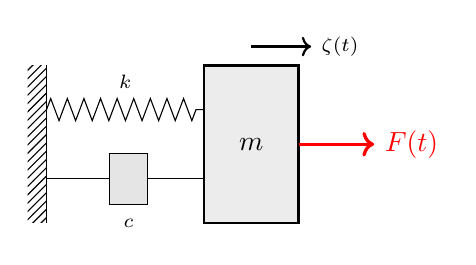
\begin{tikzpicture}[scale=0.8]
  % Wall
  \fill [pattern = north east lines] (-0.3,0) rectangle (0,2.5);
  \draw (0,0) -- (0,2.5);
  % Spring
  \draw [decorate, decoration={zigzag, segment length=6, amplitude=4}]
        (0,1.8) -- (2.5,1.8) node[midway,above=4pt] {\scriptsize $k$};
  % Damper
  \draw (0,0.7) -- (1,0.7);
  \draw[fill=gray!20] (1,0.3) rectangle (1.6,1.1);
  \draw (1.6,0.7) -- (2.5,0.7);
  \node at (1.3,0.0) {\scriptsize $c$};
  % Mass
  \draw[fill=gray!15, thick] (2.5,0) rectangle (4,2.5);
  \node at (3.25,1.25) {$m$};
  % Force
  \draw[->, very thick, red] (4,1.25) -- (5.2,1.25)
        node[right] {$F(t)$};
  % Displacement
  \draw[->, thick] (3.25,2.8) -- (4.2,2.8)
        node[right] {\scriptsize $\zeta(t)$};
\end{tikzpicture}
\end{center}
\end{column}
\begin{column}{0.58\textwidth}
Equation of motion:
\[
m\ddot{\zeta}+c\dot{\zeta}+k\zeta=F(t).
\]

Choose $x_1=\zeta,\; x_2=\dot{\zeta},\; u=F(t)$.

\begin{align*}
\dot{x}_1 &= x_2,\\
\dot{x}_2 &= -\frac{k}{m}x_1-\frac{c}{m}x_2+\frac{1}{m}u.
\end{align*}

Hence
\[
A=
\begin{bmatrix}
0 & 1\\[3pt]
-\frac{k}{m} & -\frac{c}{m}
\end{bmatrix},
\;
B=
\begin{bmatrix}
0\\[3pt]
\frac{1}{m}
\end{bmatrix},
\;
C=\begin{bmatrix}1 & 0\end{bmatrix}.
\]
\end{column}
\end{columns}
\end{frame}

% =============================================================
\section{Nonlinear systems and local linearisation}

% =============================================================
\begin{frame}{Why nonlinear systems matter}
Many practical systems are nonlinear.
Sources of nonlinearity include:
\begin{itemize}
  \item trigonometric geometry (pendulum, robotics),
  \item saturation and dead-zones (actuators),
  \item aerodynamic drag,
  \item chemical reaction kinetics,
  \item friction effects.
\end{itemize}

Key differences from linear systems:
\begin{itemize}
  \item may have \textbf{multiple equilibria},
  \item \textbf{superposition does not apply},
  \item behaviour depends strongly on the \textbf{operating point}.
\end{itemize}

For MPC, we commonly operate near a desired steady state and use
\textbf{linearisation} to obtain a local LTI approximation.
\end{frame}

% =============================================================
\begin{frame}{Equilibrium points}
An equilibrium is a state of operation where the system ceases to evolve.

\begin{defnbox}{Continuous-time equilibrium}
For $\dot{x}=f(x,u)$, a pair $(x_e,u_e)$ is an equilibrium if
\[
f(x_e,u_e)=0.
\]
\end{defnbox}

\begin{defnbox}{Discrete-time equilibrium (fixed point)}
For $x_{k+1}=f(x_k,u_k)$, a pair $(x_e,u_e)$ is an equilibrium if
\[
x_e = f(x_e,u_e).
\]
\end{defnbox}

\textbf{Physical examples:}
mechanical rest position, constant DC voltages/currents,
chemical reactor at steady state.
\end{frame}

% =============================================================
\begin{frame}{Local linearisation: Taylor expansion (scalar case)}
Consider $\dot{x}=f(x,u)$ and equilibrium $(x_e,u_e)$.

First-order Taylor expansion:
\[
f(x,u)\approx
\underbrace{f(x_e,u_e)}_{=\,0}
+\frac{\partial f}{\partial x}\Big|_{(x_e,u_e)}\!(x-x_e)
+\frac{\partial f}{\partial u}\Big|_{(x_e,u_e)}\!(u-u_e).
\]

Since $f(x_e,u_e)=0$ at equilibrium:
\[
\dot{x}\approx
\frac{\partial f}{\partial x}\Big|_{(x_e,u_e)}\!(x-x_e)
+
\frac{\partial f}{\partial u}\Big|_{(x_e,u_e)}\!(u-u_e).
\]

This is a \textbf{linear approximation} of the nonlinear system near the
equilibrium.
\end{frame}

% =============================================================
\begin{frame}{Multivariable Jacobian linearisation}
For $\dot{x}=f(x,u)$, $x\in\R^n$, $u\in\R^m$, the linearised model about
$(x_e,u_e)$ is
\[
\dot{\tilde{x}}=A\tilde{x}+B\tilde{u},
\]
where the deviation variables are
$\tilde{x}=x-x_e$, $\tilde{u}=u-u_e$,
and the Jacobians are
\[
A=\left.\frac{\partial f}{\partial x}\right|_{(x_e,u_e)}
\!=\!
\begin{bmatrix}
\frac{\partial f_1}{\partial x_1} & \cdots &
\frac{\partial f_1}{\partial x_n}\\
\vdots & \ddots & \vdots\\
\frac{\partial f_n}{\partial x_1} & \cdots &
\frac{\partial f_n}{\partial x_n}
\end{bmatrix}_{(x_e,u_e)}\!\!\!,
\quad
B=\left.\frac{\partial f}{\partial u}\right|_{(x_e,u_e)}
\!=\!
\begin{bmatrix}
\frac{\partial f_1}{\partial u_1} & \cdots &
\frac{\partial f_1}{\partial u_m}\\
\vdots & \ddots & \vdots\\
\frac{\partial f_n}{\partial u_1} & \cdots &
\frac{\partial f_n}{\partial u_m}
\end{bmatrix}_{(x_e,u_e)}\!\!\!.
\]
\end{frame}

% =============================================================
\begin{frame}{Output linearisation}
If the output map is nonlinear, $y=h(x,u)$, then its first-order expansion
gives
\[
\tilde{y}=C\tilde{x}+D\tilde{u},
\]
where
\[
C=\left.\frac{\partial h}{\partial x}\right|_{(x_e,u_e)},
\qquad
D=\left.\frac{\partial h}{\partial u}\right|_{(x_e,u_e)}.
\]

The full linearised model is therefore
\begin{align*}
\dot{\tilde{x}} &= A\tilde{x}+B\tilde{u},\\
\tilde{y} &= C\tilde{x}+D\tilde{u}.
\end{align*}

\begin{alertbox}{Validity}
This approximation is only accurate \textbf{near} the equilibrium.
Accuracy degrades as $\|\tilde{x}\|$ and $\|\tilde{u}\|$ increase.
\end{alertbox}
\end{frame}

% =============================================================
\begin{frame}{Example: planar duorotor --- nonlinear dynamics}
\begin{columns}[T,totalwidth=\textwidth]
\begin{column}{0.52\textwidth}
State vector:
\[
x=
\begin{bmatrix}
p_x & p_y & \theta & \dot{p}_x & \dot{p}_y & \dot{\theta}
\end{bmatrix}\T.
\]

Nonlinear dynamics:
\begin{align*}
\dot{x}_1 &= x_4, \quad
\dot{x}_2 = x_5, \quad
\dot{x}_3 = x_6,\\
\dot{x}_4 &= -\tfrac{1}{m}(u_1+u_2)\sin x_3,\\
\dot{x}_5 &= \tfrac{1}{m}(u_1+u_2)\cos x_3 - g,\\
\dot{x}_6 &= \tfrac{\ell}{2J}(u_2-u_1).
\end{align*}
\end{column}
\begin{column}{0.46\textwidth}
\begin{center}
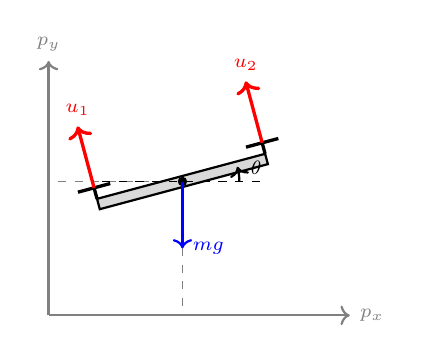
\begin{tikzpicture}[scale=0.85]
  \def\angle{15}
  \def\px{2}
  \def\py{2}
  \def\arm{1.3}
  \draw[->, thick, gray] (0,0) -- (4.5,0) node[right] {\scriptsize $p_x$};
  \draw[->, thick, gray] (0,0) -- (0,3.8) node[above] {\scriptsize $p_y$};
  \draw[dashed, gray] (\px,\py) -- (\px,0);
  \draw[dashed, gray] (\px,\py) -- (0,\py);
  \begin{scope}[shift={(\px,\py)}, rotate=\angle]
    \draw[thick, fill=gray!30] (-\arm,-0.08) rectangle (\arm,0.08);
    \node[circle, fill=black, inner sep=1.2pt] at (0,0) {};
    \draw[very thick] (-\arm,0.08) -- (-\arm,0.25);
    \draw[very thick] (-\arm-0.25,0.25) -- (-\arm+0.25,0.25);
    \draw[->, very thick, red] (-\arm,0.25) -- (-\arm,1.2)
          node[above] {\scriptsize $u_1$};
    \draw[very thick] (\arm,0.08) -- (\arm,0.25);
    \draw[very thick] (\arm-0.25,0.25) -- (\arm+0.25,0.25);
    \draw[->, very thick, red] (\arm,0.25) -- (\arm,1.2)
          node[above] {\scriptsize $u_2$};
  \end{scope}
  \draw[dashed] (\px-1.2,\py) -- (\px+1.2,\py);
  \draw[->, thick] (\px+0.85,\py) arc (0:\angle:0.85);
  \node at (\px+1.1,\py+0.2) {\scriptsize $\theta$};
  \draw[->, thick, blue] (\px,\py) -- (\px,\py-1)
        node[right] {\scriptsize $mg$};
\end{tikzpicture}
\end{center}
\end{column}
\end{columns}
\end{frame}

% =============================================================
\begin{frame}{Duorotor: hover equilibrium and linearised model}
At hover: $x_e=\mathbf{0}$, $u_{1,e}=u_{2,e}=mg/2$.

Key Jacobian entries evaluated at hover:
\[
\frac{\partial \dot{x}_4}{\partial x_3}\bigg|_{\text{eq}}
=-\frac{mg}{m}\cos(0)=-g,
\qquad
\frac{\partial \dot{x}_5}{\partial x_3}\bigg|_{\text{eq}}
=-\frac{mg}{m}\sin(0)=0.
\]

Linearised model $\dot{\tilde{x}}=A\tilde{x}+B\tilde{u}$:
\[
A=
\begin{bmatrix}
0 & 0 & 0 & 1 & 0 & 0\\
0 & 0 & 0 & 0 & 1 & 0\\
0 & 0 & 0 & 0 & 0 & 1\\
0 & 0 & -g & 0 & 0 & 0\\
0 & 0 & 0 & 0 & 0 & 0\\
0 & 0 & 0 & 0 & 0 & 0
\end{bmatrix},
\quad
B=
\begin{bmatrix}
0 & 0\\
0 & 0\\
0 & 0\\
0 & 0\\
\frac{1}{m} & \frac{1}{m}\\[3pt]
-\frac{\ell}{2J} & \frac{\ell}{2J}
\end{bmatrix}.
\]
\end{frame}

% =============================================================
\section{Discretisation of CT systems}

% =============================================================
\begin{frame}{Exact solution of a homogeneous LTI system}
For the autonomous LTI system $\dot{x}(t)=Ax(t)$,
the exact solution over interval $\Delta t$ is
\[
x(t+\Delta t)=e^{A\Delta t}\,x(t).
\]

The \textbf{matrix exponential} is defined by the Taylor series:
\[
e^{M}= I + M + \frac{1}{2!}M^2 + \frac{1}{3!}M^3 + \cdots
\]

\begin{notebox}{Practical MATLAB note}
Use \texttt{expm(A*h)} to compute the matrix exponential numerically.
Do \textbf{not} use \texttt{exp(A*h)} (element-wise exponential).
\end{notebox}
\end{frame}

% =============================================================
\begin{frame}{Exact discretisation vs numerical approximation}
With sampling time $h$:
\[
x_{k+1}=A_d\,x_k, \qquad A_d = e^{Ah}.
\]

This is the \textbf{exact} discrete-time realisation---not an approximation.

\begin{center}
\renewcommand{\arraystretch}{1.3}
\begin{tabular}{|p{0.42\textwidth}|p{0.42\textwidth}|}
\hline
\textbf{Linear systems} & \textbf{Nonlinear systems}\\
\hline
$\dot{x}=Ax$ & $\dot{x}=f(x)$\\
Solved exactly via $e^{Ah}$ & Almost never have closed-form solutions\\
Discretised exactly & Discretised approximately (Euler, RK4, \ldots)\\
\hline
\end{tabular}
\end{center}
\end{frame}

% =============================================================
\begin{frame}{Zero-Order Hold (ZOH) discretisation of forced systems}
For $\dot{x}=Ax+Bu$, assume the input is held constant between samples:
\[
u(t)=u_k,\qquad t\in[t_k,\,t_{k+1}).
\]

\textbf{Augmented-state trick:}
Under ZOH, $\dot{u}=0$, so define $z=[x\T\;\;u\T]\T$:
\[
\dot{z}=
\underbrace{
\begin{bmatrix}
A & B\\ 0 & 0
\end{bmatrix}}_{T}\,z.
\]

Apply the matrix exponential:
\[
e^{Th}=
\begin{bmatrix}
A_d & B_d\\ 0 & I
\end{bmatrix}
\quad\Longrightarrow\quad
\boxed{x_{k+1}=A_d\,x_k + B_d\,u_k}.
\]

This is the exact discrete-time model used in linear MPC prediction.
\end{frame}

% =============================================================
\begin{frame}[fragile]{MATLAB code for exact ZOH discretisation}
\begin{lstlisting}[caption={Exact ZOH discretisation using the augmented matrix exponential.}]
% Define a continuous-time LTI system
A = [0, 1; -5, -2];   % Example A matrix
B = [0; 1];            % Example B matrix
h = 0.1;               % Sampling time (s)

n = size(A, 1);   % Number of states
m = size(B, 2);   % Number of inputs

% Form the augmented matrix T
T = [A, B;
     zeros(m,n), zeros(m,m)];

% Compute the matrix exponential of T*h
M = expm(T * h);

% Extract the discrete-time matrices
Ad = M(1:n, 1:n);
Bd = M(1:n, n+1:end);

disp('Ad = '); disp(Ad);
disp('Bd = '); disp(Bd);
\end{lstlisting}
\end{frame}

% =============================================================
\section{Numerical discretisation of nonlinear systems}

% =============================================================
\begin{frame}{Forward Euler method}
For a nonlinear system $\dot{x}=f(x,u)$, the simplest numerical
integration is
\[
x_{k+1}=x_k + h\,f(x_k,u_k).
\]

\textbf{Pros:} simple, cheap, easy to differentiate.

\textbf{Cons:} only first-order accurate ($\mathcal{O}(h)$), poor
stability, can introduce artificial energy.

\begin{alertbox}{Warning}
Forward Euler is often too crude for accurate plant simulation.
It can cause stable systems to \textbf{appear unstable} by injecting
artificial energy.  Prefer RK4 for engineering work.
\end{alertbox}
\end{frame}

% =============================================================
\begin{frame}{Runge--Kutta 4 (RK4) method}
RK4 evaluates the slope \textbf{four times} per step:
\begin{align*}
k_1 &= f(x_k,\,u_k),\\
k_2 &= f\!\left(x_k+\tfrac{h}{2}k_1,\,u_k\right),\\
k_3 &= f\!\left(x_k+\tfrac{h}{2}k_2,\,u_k\right),\\
k_4 &= f(x_k+h\,k_3,\,u_k),
\end{align*}
then forms the weighted update:
\[
\boxed{x_{k+1}=x_k+\frac{h}{6}\big(k_1+2k_2+2k_3+k_4\big)}.
\]

Global error: $\mathcal{O}(h^4)$ --- much more accurate than Euler for the same
step size.  RK4 is the \textbf{standard workhorse} of engineering
simulation.
\end{frame}

% =============================================================
\begin{frame}[fragile]{MATLAB implementation of one RK4 step}
\begin{lstlisting}[caption={Generic MATLAB function for one RK4 step.}]
function x_next = rk4_step(f_dynamics, x_curr, u_curr, h)
    % f_dynamics: function handle @(x,u) returning dx/dt
    % x_curr:     current state vector [n x 1]
    % u_curr:     current input vector [m x 1]
    % h:          time step (dt)

    k1 = f_dynamics(x_curr, u_curr);
    k2 = f_dynamics(x_curr + 0.5*h*k1, u_curr);
    k3 = f_dynamics(x_curr + 0.5*h*k2, u_curr);
    k4 = f_dynamics(x_curr + h*k3, u_curr);

    x_next = x_curr + (h/6)*(k1 + 2*k2 + 2*k3 + k4);
end
\end{lstlisting}
\end{frame}

% =============================================================
\begin{frame}{Comparison: Euler vs RK4 on a harmonic oscillator}
\begin{columns}[T,totalwidth=\textwidth]
\begin{column}{0.48\textwidth}
Undamped mass-spring: $\ddot{p}+p=0$,
$x=[p,\;\dot{p}]\T$,
\[
\dot{x}=\begin{bmatrix}x_2\\-x_1\end{bmatrix}.
\]

Exact solution: $x_1(t)=\cos(t)$ (sinusoid,
energy conserved, circular phase portrait).

\medskip
\textbf{Euler:} spirals outward (artificial energy injection).

\textbf{RK4:} tracks the true oscillation faithfully even at larger $h$.
\end{column}
\begin{column}{0.50\textwidth}
\begin{center}
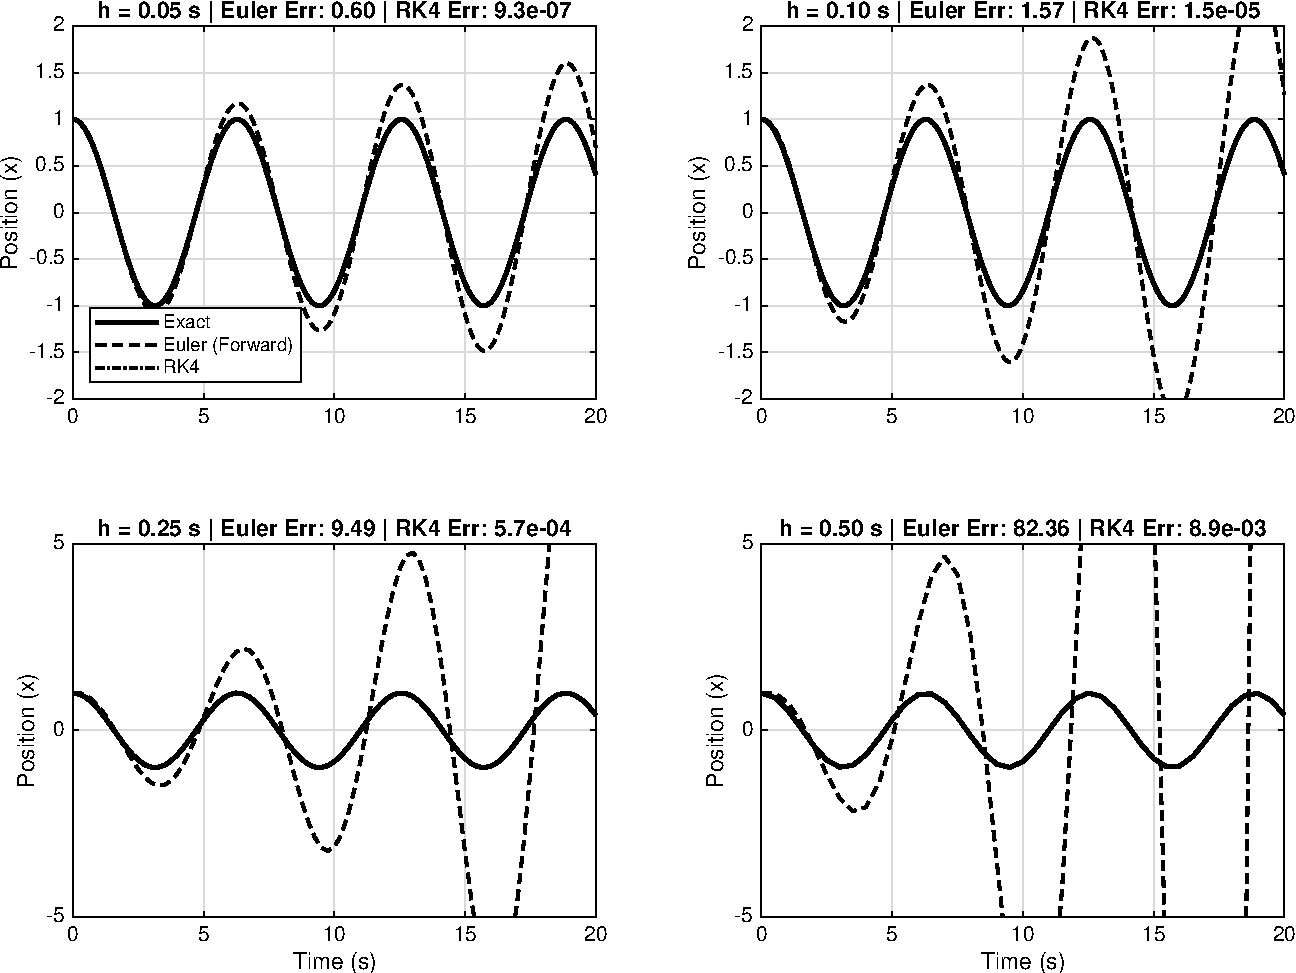
\includegraphics[width=\linewidth,height=0.7\textheight,keepaspectratio]{RK4_vs_euler.pdf}
\end{center}
\end{column}
\end{columns}
\end{frame}

% =============================================================
\section{Stability of discrete-time systems}

% =============================================================
\begin{frame}{Discrete-time stability condition}
For the discrete-time system $x_{k+1}=A_d\,x_k$,
the equilibrium at the origin is asymptotically stable iff
every eigenvalue of $A_d$ lies strictly inside the unit circle:
\[
|\lambda_i(A_d)|<1,\qquad \forall\;i.
\]

\begin{columns}[T,totalwidth=\textwidth]
\begin{column}{0.50\textwidth}
\begin{alertbox}{Stability test summary}
Inside unit circle $\Rightarrow$ asymptotically stable.\\
On unit circle $\Rightarrow$ marginal.\\
Outside unit circle $\Rightarrow$ unstable.
\end{alertbox}
\end{column}
\begin{column}{0.48\textwidth}
\begin{center}
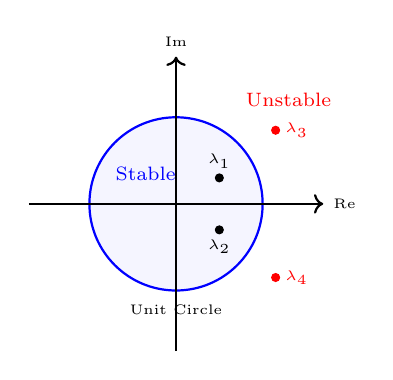
\begin{tikzpicture}[scale=1.1]
  \draw[thick, blue, fill=blue!4] (0,0) circle (1cm);
  \node[blue, font=\scriptsize] at (-0.35,0.35) {Stable};
  \node[red, font=\scriptsize] at (1.3,1.2) {Unstable};
  \filldraw[black] (0.5,0.3) circle (1.3pt)
        node[above, font=\tiny] {$\lambda_1$};
  \filldraw[black] (0.5,-0.3) circle (1.3pt)
        node[below, font=\tiny] {$\lambda_2$};
  \filldraw[red] (1.15,0.85) circle (1.3pt)
        node[right, font=\tiny] {$\lambda_3$};
  \filldraw[red] (1.15,-0.85) circle (1.3pt)
        node[right, font=\tiny] {$\lambda_4$};
  \node[anchor=north, font=\tiny] at (0,-1.05) {Unit Circle};
  \draw[->, thick] (-1.7,0) -- (1.7,0) node[right, font=\tiny] {Re};
  \draw[->, thick] (0,-1.7) -- (0,1.7) node[above, font=\tiny] {Im};
\end{tikzpicture}
\end{center}
\end{column}
\end{columns}
\end{frame}

% =============================================================
\begin{frame}{Continuous-time vs discrete-time stability mapping}
The mapping between $s$-plane and $z$-plane poles is
\[
z = e^{sT},
\]
where $T$ is the sampling period.

\medskip
Consequences:
\begin{itemize}
  \item Left half-plane in $s$ $\longleftrightarrow$ inside unit circle in $z$.
  \item Imaginary axis $\longleftrightarrow$ unit circle.
  \item Right half-plane $\longleftrightarrow$ outside unit circle.
\end{itemize}

\begin{notebox}{Practical point}
Always check stability in the \textbf{correct domain} (CT vs DT) for the
model you are actually using.
\end{notebox}
\end{frame}

% =============================================================
\begin{frame}{Lyapunov stability and the Stein equation}
Define the quadratic ``energy'' candidate:
\[
V(x_k)=x_k\T P\,x_k,\qquad P\succ 0.
\]

For $x_{k+1}=Ax_k$:
\[
V(x_{k+1})-V(x_k)
= x_k\T\!\big(A\T PA - P\big)x_k.
\]

Energy decreases iff $A\T PA - P \prec 0$.

\begin{alertbox}{Discrete Lyapunov theorem (Stein equation)}
$x_{k+1}=Ax_k$ is asymptotically stable iff, for any $Q\succ 0$, there
exists a unique $P\succ 0$ satisfying
\[
A\T PA - P = -Q.
\]
\end{alertbox}

\begin{notebox}{Connection to LQR}
In LQR / MPC, we shape $A_{cl}=A-BK$ so that this energy-decrease
condition is satisfied optimally.
\end{notebox}
\end{frame}

% =============================================================
\begin{frame}{Part I summary: state-space modelling}
\begin{itemize}
  \item State-space models describe dynamics through internal variables (states).
  \item States usually arise from stored energy (positions, velocities, currents, voltages).
  \item Nonlinear models are linearised locally around equilibria using Jacobians.
  \item CT LTI systems are discretised \textbf{exactly} via the matrix exponential (ZOH):
  \[
  x_{k+1}=A_d\,x_k+B_d\,u_k.
  \]
  \item Nonlinear systems require approximate numerical integration; RK4 $\gg$ Euler.
  \item DT stability: all eigenvalues inside the unit circle.
\end{itemize}

\begin{summarybox}{Bridge to the next part}
Now that we have the modelling framework, the next question is:
\textbf{can we actually control and observe this system?}
\end{summarybox}
\end{frame}

% #############################################################
%  PART II: CONTROLLABILITY & OBSERVABILITY  (Chapter 4)
% #############################################################

\part{Controllability \& Observability}

\section{Motivation: existence conditions for control}

% =============================================================
\begin{frame}{Why do we need controllability and observability?}
In previous chapters we focused on \textbf{optimisation}: choosing the
best input sequence to minimise a cost.

Before asking \emph{``what is optimal?''} we must ask something more
fundamental:

\begin{center}
\textbf{Does a feasible trajectory even exist?}
\end{center}

Two structural properties answer this:
\begin{itemize}
  \item \textbf{Controllability} (actuation): can inputs steer the state
        where we want?
  \item \textbf{Observability} (sensing): can outputs reveal the
        internal state?
\end{itemize}

\begin{alertbox}{Key message}
If a system is uncontrollable or unobservable, \textbf{no} sophisticated
MPC/LQR algorithm can overcome that limitation.
\end{alertbox}
\end{frame}

% =============================================================
\begin{frame}{Controllability vs observability: the twin questions}
\begin{columns}[T,totalwidth=\textwidth]
\begin{column}{0.49\textwidth}
\begin{defnbox}{Controllability (actuation)}
Given $x_{k+1}=Ax_k+Bu_k$, can we steer from \emph{any} $x_0$ to
\emph{any} target $x_N$ using a finite input sequence?
\end{defnbox}
\vspace{0.2em}
\begin{itemize}
  \item depends on the pair $(A,B)$
  \item about \emph{reachability} of states
  \item prerequisite for controller design
\end{itemize}
\end{column}
\begin{column}{0.49\textwidth}
\begin{defnbox}{Observability (sensing)}
Given $y_k=Cx_k+Du_k$, can we uniquely reconstruct $x_0$ from knowledge
of $u$ and $y$ over a finite horizon?
\end{defnbox}
\vspace{0.2em}
\begin{itemize}
  \item depends on the pair $(A,C)$
  \item about \emph{information flow} to sensors
  \item prerequisite for observer / Kalman filter
\end{itemize}
\end{column}
\end{columns}
\end{frame}

% =============================================================
\section{Controllability}

% =============================================================
\begin{frame}{Controllability: the core question}
Given the discrete-time LTI model
\[
x_{k+1}=Ax_k+Bu_k,
\]
the fundamental question is:

\begin{center}
\emph{Do the actuators (matrix $B$) have sufficient authority to influence
\textbf{all} state directions governed by $A$?}
\end{center}

\begin{itemize}
  \item If $B=0$, then $u_k$ has no effect $\Rightarrow$ uncontrollable.
  \item Even with $B\neq 0$, actuation may be restricted to a
        \textbf{subspace} of $\R^n$.
\end{itemize}

\begin{defnbox}{Definition: Controllability}
A system is \emph{controllable} if, for any $x_0$ and any $x_N$, there
exists a finite input sequence $\{u_0,\ldots,u_{N-1}\}$ that drives the
system from $x_0$ to $x_N$.
\end{defnbox}
\end{frame}

% =============================================================
\subsection{Derivation of the rank condition}

% =============================================================
\begin{frame}{Expanding the dynamics (recursive substitution)}
Starting from $x_{k+1}=Ax_k+Bu_k$, expand step by step:
\begin{align*}
x_1 &= Ax_0+Bu_0,\\
x_2 &= A^2x_0 + ABu_0 + Bu_1,\\
&\;\vdots\\
x_N &= A^N x_0 + \sum_{i=0}^{N-1} A^{N-1-i}B\,u_i.
\end{align*}

Rearranging:
\[
\underbrace{x_N - A^N x_0}_{b}
=
\underbrace{\begin{bmatrix}
B & AB & A^2B & \cdots & A^{N-1}B
\end{bmatrix}}_{\Ccal_N}
\underbrace{\begin{bmatrix}
u_{N-1}\\ u_{N-2}\\ \vdots\\ u_0
\end{bmatrix}}_{\mathcal{U}}.
\]

This is a linear system $b=\Ccal_N\,\mathcal{U}$.
\end{frame}

% =============================================================
\begin{frame}{Controllability as a solvability problem}
\begin{alertbox}{Key question}
Does a solution $\mathcal{U}$ exist for \emph{any} desired vector
$b\in\R^n$?
\end{alertbox}

This holds iff the columns of $\Ccal_N$ span $\R^n$, i.e.\
$\mathrm{rank}(\Ccal_N)=n$.

But $\Ccal_N$ grows with $N$.  We need a \textbf{finite} test.

\begin{notebox}{Cayley--Hamilton theorem}
Any matrix power $A^k$ for $k\ge n$ is a linear combination of
$I,A,\ldots,A^{n-1}$.  Therefore columns beyond $A^{n-1}B$ add \textbf{no
new independent directions}.
\end{notebox}

Standard controllability matrix:
\[
\Ccal = \begin{bmatrix}
B & AB & A^2B & \cdots & A^{n-1}B
\end{bmatrix}.
\]
\end{frame}

% =============================================================
\begin{frame}{Kalman rank condition (controllability)}
\begin{alertbox}{Theorem: Kalman rank condition}
The pair $(A,B)$ is controllable if and only if
\[
\mathrm{rank}(\Ccal)=n,
\qquad
\Ccal=\begin{bmatrix}B & AB & \cdots & A^{n-1}B\end{bmatrix}.
\]
\end{alertbox}

\textbf{Interpretation:}
\begin{itemize}
  \item The columns of $\Ccal$ span the entire state space $\R^n$.
  \item There is no ``hidden'' subspace immune to actuation.
  \item The input $u$ has authority to steer the state anywhere.
\end{itemize}

\begin{notebox}{Important caveat}
Controllability is a \textbf{structural} (existence) condition.  It does not
guarantee easy control---actuator constraints, long horizons, and poor
conditioning can still make practical control very difficult.
\end{notebox}
\end{frame}

% =============================================================
\begin{frame}{Controllability decomposition (geometric view)}
\begin{center}
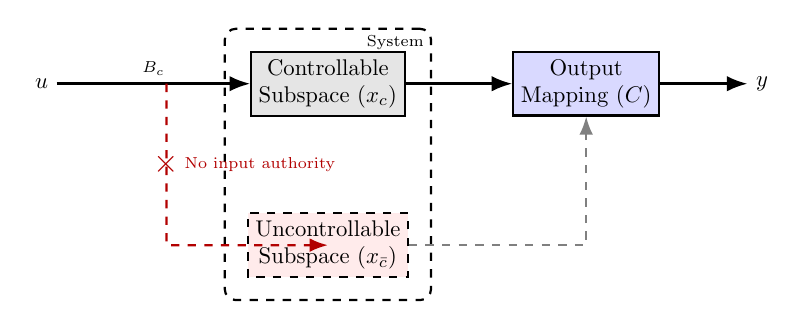
\begin{tikzpicture}[auto, >=Latex, thick, scale=0.82, transform shape]
  \tikzstyle{block} = [draw, rectangle, fill=gray!20,
        minimum height=2.5em, minimum width=5em, align=center]
  \tikzstyle{dashedblock} = [draw, dashed, rectangle, fill=red!8,
        minimum height=2.5em, minimum width=5em, align=center]
  \tikzstyle{line} = [draw, ->]
  \tikzstyle{bigbox} = [draw, dashed, rounded corners, inner sep=8pt]

  \node [coordinate] (input) at (-1.2, 0) {};
  \node [left] at (input) {$u$};

  \node [block] (controllable) at (3, 0)
        {Controllable\\Subspace ($x_c$)};
  \node [dashedblock] (uncontrollable) at (3, -2.5)
        {Uncontrollable\\Subspace ($x_{\bar{c}}$)};
  \node [block, fill=blue!15] (output_map) at (7, 0)
        {Output\\Mapping ($C$)};
  \node [coordinate] (output) at (9.5, 0) {};
  \node [right] at (output) {$y$};

  \node [bigbox, fit=(controllable)(uncontrollable),
         label={[anchor=north east, font=\scriptsize]north east:System}] {};

  \draw [line, line width=1pt] (input) -- node[above]{\scriptsize$B_c$}
        (controllable);
  \draw [line, line width=1pt] (controllable) -- (output_map);
  \draw [line, line width=1pt] (output_map) -- (output);
  \draw [line, dashed, gray] (uncontrollable) -| (output_map);

  \draw [line, dashed, red!70!black] (0.5, 0) -- (0.5, -2.5)
        -- (controllable |- uncontrollable.west);
  \node [red!70!black, font=\Large\bfseries] at (0.5, -1.25) {$\times$};
  \node [red!70!black, font=\scriptsize, right] at (0.65, -1.25)
        {No input authority};
\end{tikzpicture}
\end{center}

The Kalman decomposition separates the state space into controllable and
uncontrollable parts.  Only $x_c$ can be steered by $u$.  The
uncontrollable subspace evolves independently.
\end{frame}

% =============================================================
\begin{frame}{Example: triple integrator ($n=3$)}
\[
A = \begin{bmatrix} 0 & 1 & 0 \\ 0 & 0 & 1 \\ 0 & 0 & 0 \end{bmatrix},
\qquad
B = \begin{bmatrix} 0 \\ 0 \\ 1 \end{bmatrix}.
\]

Compute $\Ccal = [B \;\; AB \;\; A^2B]$:
\[
AB = \begin{bmatrix}0\\1\\0\end{bmatrix},
\quad
A^2B = \begin{bmatrix}1\\0\\0\end{bmatrix},
\quad
\Ccal = \begin{bmatrix}
0 & 0 & 1\\
0 & 1 & 0\\
1 & 0 & 0
\end{bmatrix}.
\]

$\det(\Ccal) = -1 \neq 0$
$\;\Rightarrow\;$ $\mathrm{rank}(\Ccal)=3=n$
$\;\Rightarrow\;$ \textbf{controllable}.

\begin{notebox}{Interpretation}
Despite $u$ entering only the 3rd state equation, its effect propagates
through the chain of integrators: after 1 step it reaches $x_3$, after 2
steps $x_2$, and after 3 steps $x_1$.  This is the \emph{controllable
canonical form}.
\end{notebox}
\end{frame}

% =============================================================
\subsection{Controllability in MATLAB}

\begin{frame}[fragile]{MATLAB: controllability check with \texttt{ctrb}}
\begin{lstlisting}[caption={Checking controllability of a double integrator.}]
% Discrete-time double integrator
h = 0.1;
A = [1, h;
     0, 1];
B = [0.5*h^2;
     h];
n = size(A, 1);

% Compute Controllability Matrix
Co = ctrb(A, B);
rank_Co = rank(Co);

fprintf('State dimension n = %d\n', n);
fprintf('Rank of Co       = %d\n', rank_Co);

if rank_Co == n
    fprintf('System is CONTROLLABLE.\n');
else
    fprintf('System is NOT controllable.\n');
end
\end{lstlisting}

For the double integrator: $\mathrm{rank}(\Ccal)=2=n$ $\Rightarrow$ controllable.
\end{frame}

% =============================================================
\section{Observability}

% =============================================================
\begin{frame}{Observability: the inverse problem}
\begin{itemize}
  \item \textbf{Controllability:} choose $u$ to \textbf{affect} $x$.
  \item \textbf{Observability:} use $u$ and $y$ to \textbf{infer} $x$.
\end{itemize}

Most advanced controllers require full state feedback (or a state
estimate):
\[
u_k = -K\hat{x}_k
\quad\text{or}\quad
u_k = \pi(\hat{x}_k).
\]

If not all states are measured, we need a \textbf{state observer} (e.g.\
Kalman filter).
Observability tells us whether this reconstruction is possible.

\begin{defnbox}{Definition: Observability}
A linear system is \textbf{observable} if the initial state $x(t_0)$ can
be uniquely determined from knowledge of $u(t)$ and $y(t)$ over a finite
time interval.
\end{defnbox}
\end{frame}

% =============================================================
\subsection{The observability matrix}

\begin{frame}{The observability matrix and rank condition}
For an LTI system, define
\[
\Ocal=
\begin{bmatrix}
C\\ CA\\ CA^2\\ \vdots\\ CA^{n-1}
\end{bmatrix}
\in\R^{np\times n}.
\]

\begin{alertbox}{Kalman rank condition (observability)}
The pair $(A,C)$ is observable iff
\[
\mathrm{rank}(\Ocal)=n.
\]
\end{alertbox}

If the rank is less than $n$, some state directions are ``hidden''---they
leave no trace in the output, and the observer cannot reconstruct them.
\end{frame}

% =============================================================
\subsection{Derivation via stacking measurements}

\begin{frame}{Deriving the test: stacking output measurements}
For the unforced system $x_{k+1}=Ax_k$, $y_k=Cx_k$:
\begin{align*}
y_0 &= Cx_0,\\
y_1 &= CAx_0,\\
y_2 &= CA^2x_0,\\
&\;\vdots\\
y_{n-1} &= CA^{n-1}x_0.
\end{align*}

Stacking:
\[
\underbrace{\begin{bmatrix}
y_0\\ y_1\\ \vdots\\ y_{n-1}
\end{bmatrix}}_{Y}
=
\underbrace{\begin{bmatrix}
C\\ CA\\ \vdots\\ CA^{n-1}
\end{bmatrix}}_{\Ocal}
x_0.
\]

If $\mathrm{rank}(\Ocal)=n$, we can solve uniquely:
$x_0 = (\Ocal\T\Ocal)^{-1}\Ocal\T Y$.

By Cayley--Hamilton, measurements beyond $k=n{-}1$ add no new information.
\end{frame}

% =============================================================
\begin{frame}{Example: an unobservable system}
\[
\dot{x}=\begin{bmatrix}-1&0\\0&-2\end{bmatrix}x+\begin{bmatrix}1\\1\end{bmatrix}u,
\qquad
y=\begin{bmatrix}1&0\end{bmatrix}x.
\]

Compute:
\[
\Ocal=\begin{bmatrix}C\\CA\end{bmatrix}
=\begin{bmatrix}1&0\\-1&0\end{bmatrix}.
\]

Second column is entirely zero $\Rightarrow$ $x_2$ never affects $y$.
\[
\mathrm{rank}(\Ocal)=1<2 \quad\Rightarrow\quad \textbf{not observable}.
\]

\begin{alertbox}{Danger}
If the unobservable mode $x_2$ were unstable, the system could diverge
internally while the output $y$ shows no warning.  The controller would be
\textbf{blind} to the instability.
\end{alertbox}
\end{frame}

% =============================================================
\begin{frame}{Fixing observability: changing the sensor}
Same system, but now $C=\begin{bmatrix}1&1\end{bmatrix}$ (sensor measures
$y=x_1+x_2$):

\[
CA=\begin{bmatrix}1&1\end{bmatrix}
\begin{bmatrix}-1&0\\0&-2\end{bmatrix}
=\begin{bmatrix}-1&-2\end{bmatrix}.
\]
\[
\Ocal=\begin{bmatrix}1&1\\-1&-2\end{bmatrix},
\qquad
\det(\Ocal)=(1)(-2)-(1)(-1)=-1\neq 0.
\]

$\mathrm{rank}(\Ocal)=2=n$ $\Rightarrow$ \textbf{observable}.

\begin{notebox}{Key lesson}
Observability is a property of the \textbf{pair} $(A,C)$.
The same dynamics can be observable or unobservable depending entirely
on the sensor configuration.  Sensor choice matters enormously.
\end{notebox}
\end{frame}

% =============================================================
\subsection{Observability in MATLAB}

\begin{frame}[fragile]{MATLAB: observability check with \texttt{obsv}}
\begin{lstlisting}[caption={Comparing observability for two sensor configurations.}]
h = 0.1;
A = [1, h;
     0, 1];
n = size(A, 1);

% Case 1: position sensor
C1 = [1, 0];
Ob1 = obsv(A, C1);
rank1 = rank(Ob1);

% Case 2: velocity sensor
C2 = [0, 1];
Ob2 = obsv(A, C2);
rank2 = rank(Ob2);

fprintf('Position sensor: rank(O) = %d  =>  %s\n', ...
        rank1, char((rank1==n)*'Observable' + ...
                     (rank1<n)*'NOT observable'));
fprintf('Velocity sensor: rank(O) = %d\n', rank2);
\end{lstlisting}

\textbf{Result:} position sensor $\Rightarrow$ observable.
Velocity sensor $\Rightarrow$ NOT observable (absolute position unknown).
\end{frame}

% =============================================================
\begin{frame}{Interpreting the observability results}
\textbf{Double integrator} (position, velocity):

\medskip
\begin{center}
\renewcommand{\arraystretch}{1.3}
\begin{tabular}{lccl}
\toprule
Sensor & $C$ & $\mathrm{rank}(\Ocal)$ & Verdict \\
\midrule
Position & $[1\;\;0]$ & 2 & Observable \\
Velocity & $[0\;\;1]$ & 1 & \textbf{Not} observable \\
Both     & $\begin{bmatrix}1&0\\0&1\end{bmatrix}$ & 2 & Observable \\
\bottomrule
\end{tabular}
\end{center}

\medskip
\textbf{Intuition:}
\begin{itemize}
  \item Measuring position over time reveals velocity (by differences).
  \item Measuring velocity alone does \textbf{not} reveal absolute position
        (unknown integration constant).
\end{itemize}

\begin{notebox}{Practical takeaway}
Always check observability \textbf{before} designing a state estimator.
\end{notebox}
\end{frame}

% =============================================================
\section{Geometric intuition and the PBH test}

% =============================================================
\begin{frame}{Geometric intuition: reachable and hidden subspaces}
\begin{columns}[T,totalwidth=\textwidth]
\begin{column}{0.48\textwidth}
\begin{defnbox}{Controllability}
Columns of $\Ccal$ span the set of state directions reachable by the
input.  If this span is $\R^n$, every direction is reachable.
\end{defnbox}

\begin{center}
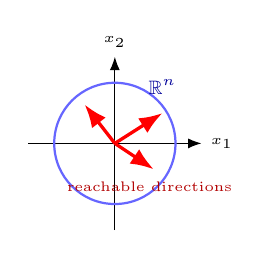
\begin{tikzpicture}[scale=0.55, >=Latex]
  \draw[->] (-2,0) -- (2,0) node[right] {\tiny $x_1$};
  \draw[->] (0,-2) -- (0,2) node[above] {\tiny $x_2$};
  \draw[thick, blue!60] (0,0) circle (1.4);
  \node[blue!60!black, font=\scriptsize] at (1.1,1.3) {$\R^n$};
  \draw[very thick, red, ->] (0,0) -- (1.1,0.7);
  \draw[very thick, red, ->] (0,0) -- (-0.7,0.9);
  \draw[very thick, red, ->] (0,0) -- (0.9,-0.6);
  \node[red!70!black, font=\tiny] at (0.8,-1.0)
        {reachable directions};
\end{tikzpicture}
\end{center}
\end{column}
\begin{column}{0.48\textwidth}
\begin{defnbox}{Observability}
If $\mathrm{rank}(\Ocal)<n$, $\exists\;v\neq 0$ with $\Ocal v=0$.
Motion along $v$ leaves \textbf{no trace} in the output.
\end{defnbox}

\begin{center}
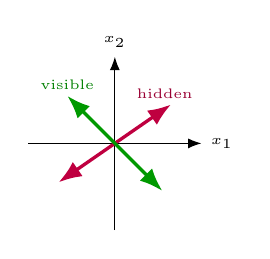
\begin{tikzpicture}[scale=0.55, >=Latex]
  \draw[->] (-2,0) -- (2,0) node[right] {\tiny $x_1$};
  \draw[->] (0,-2) -- (0,2) node[above] {\tiny $x_2$};
  \draw[very thick, purple, <->] (-1.3,-0.9) -- (1.3,0.9);
  \node[purple!80!black, font=\tiny] at (1.15,1.15) {hidden};
  \draw[very thick, green!60!black, <->] (-1.1,1.1) -- (1.1,-1.1);
  \node[green!50!black, font=\tiny] at (-1.1,1.35) {visible};
\end{tikzpicture}
\end{center}
\end{column}
\end{columns}
\end{frame}

% =============================================================
\begin{frame}{The PBH (Hautus) test}
An alternative to the rank test is the \textbf{Popov--Belevitch--Hautus}
(PBH) test, which checks controllability/observability \textbf{mode by mode}.

\begin{columns}[T,totalwidth=\textwidth]
\begin{column}{0.48\textwidth}
\begin{defnbox}{PBH: controllability}
$(A,B)$ is controllable iff
\[
\mathrm{rank}\!\begin{bmatrix}\lambda I - A & B\end{bmatrix}=n
\]
for every eigenvalue $\lambda$ of $A$.
\end{defnbox}
\end{column}
\begin{column}{0.48\textwidth}
\begin{defnbox}{PBH: observability}
$(A,C)$ is observable iff
\[
\mathrm{rank}\!\begin{bmatrix}\lambda I - A \\ C\end{bmatrix}=n
\]
for every eigenvalue $\lambda$ of $A$.
\end{defnbox}
\end{column}
\end{columns}

\vspace{0.3em}
\textbf{Advantage:} the PBH test identifies \textbf{which modes} are
uncontrollable/unobservable, not just whether the overall test passes or
fails.
\end{frame}

% =============================================================
\begin{frame}{PBH example: identifying an uncontrollable mode}
\[
A=\begin{bmatrix}-1&0\\0&-3\end{bmatrix},
\qquad
B=\begin{bmatrix}1\\0\end{bmatrix}.
\]

Eigenvalues: $\lambda_1=-1$, $\lambda_2=-3$.

\textbf{At $\lambda_1=-1$:}
\[
\begin{bmatrix}\lambda_1 I-A & B\end{bmatrix}
=\begin{bmatrix}0&0&1\\0&2&0\end{bmatrix}
\quad\Rightarrow\quad \mathrm{rank}=2=n \;\checkmark
\]

\textbf{At $\lambda_2=-3$:}
\[
\begin{bmatrix}\lambda_2 I-A & B\end{bmatrix}
=\begin{bmatrix}-2&0&1\\0&0&0\end{bmatrix}
\quad\Rightarrow\quad \mathrm{rank}=1<n \;\times
\]

The mode at $\lambda=-3$ is \textbf{uncontrollable}.  Input $u$ cannot
influence $x_2$.
\end{frame}

% =============================================================
\section{Stabilisability and detectability}

\begin{frame}{Weaker conditions: stabilisability and detectability}
In practice, MPC does not always require \textbf{full} controllability or
observability.  Weaker conditions suffice:

\begin{defnbox}{Stabilisability}
A system is \emph{stabilisable} if all \textbf{uncontrollable} modes are
\textbf{stable} (eigenvalues inside the unit circle / left half-plane).
\end{defnbox}

\begin{defnbox}{Detectability}
A system is \emph{detectable} if all \textbf{unobservable} modes are
\textbf{stable}.
\end{defnbox}

\begin{notebox}{Why this matters}
\begin{itemize}
  \item Stabilisability is sufficient for DARE solutions and LQR to exist.
  \item Detectability is sufficient for Kalman filter convergence.
  \item These weaker properties appear in MPC stability proofs (Ch.\ 5--7).
\end{itemize}
\end{notebox}
\end{frame}

% =============================================================
\section{Common pitfalls}

\begin{frame}{Common pitfalls and misconceptions}
\begin{itemize}
  \item \textbf{Controllable $\neq$ easy to control.}
        A system may require huge inputs, long horizons, or violate
        actuator constraints.

  \item \textbf{Observable $\neq$ easy to estimate.}
        A poorly conditioned $\Ocal$ leads to noisy, slow estimation.

  \item \textbf{Rank tests are structural, not performance tests.}
        They answer ``possible or impossible?'', not ``fast, robust, or
        well-conditioned?''

  \item \textbf{Sensor choice matters enormously.}
        Measuring the ``wrong'' variable can make an otherwise simple
        system unobservable.

  \item \textbf{CT and DT tests are analogous but not identical.}
        Always check the correct pair $(A,B)$ or $(A,C)$ for the model
        you are actually using.
\end{itemize}

\begin{alertbox}{Practical lesson}
Before designing an MPC controller or observer, always check
controllability / observability first.
\end{alertbox}
\end{frame}

% =============================================================
\section{Key takeaways and exercises}

\begin{frame}{Key takeaways}
\begin{itemize}
  \item Controllability and observability are \textbf{existence conditions}
        for control and estimation.
  \item Controllability matrix:
  $\Ccal=[B\;AB\;\ldots\;A^{n-1}B]$, \quad
  $\mathrm{rank}(\Ccal)=n$.
  \item Observability matrix:
  $\Ocal=[C;\;CA;\;\ldots;\;CA^{n-1}]$, \quad
  $\mathrm{rank}(\Ocal)=n$.
  \item The PBH test identifies \textbf{which modes} are
        uncontrollable / unobservable.
  \item Stabilisability and detectability are weaker but often sufficient
        conditions for MPC/LQR/Kalman filter design.
  \item If uncontrollable: some state directions \textbf{cannot} be
        influenced by input.
  \item If unobservable: some internal modes \textbf{cannot} be inferred
        from output history.
\end{itemize}

\begin{summarybox}{Bottom line}
\textbf{You cannot optimise what you cannot reach or observe.}
\end{summarybox}
\end{frame}

% =============================================================
\begin{frame}{Chapter summary: the full picture}
\begin{center}
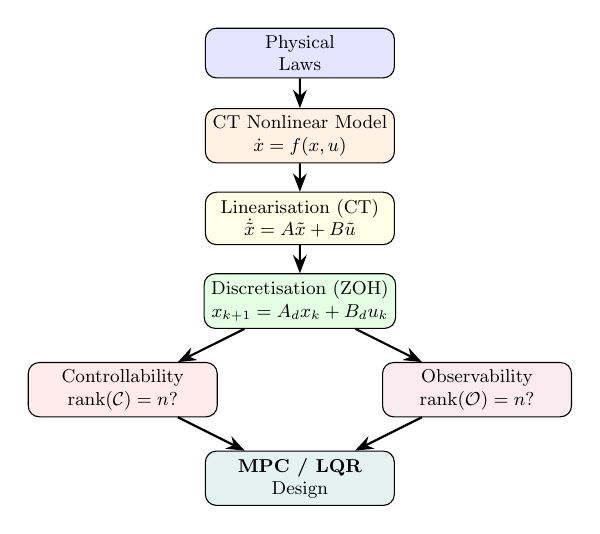
\begin{tikzpicture}[scale=0.75, transform shape,
  every node/.style={font=\small},
  box/.style={draw, rounded corners, minimum width=3.2cm,
              minimum height=0.7cm, align=center},
  arrow/.style={-Stealth, thick}
]
  % Vertical flow: Physics -> NL -> Linearise -> CT LTI -> Discretise -> DT LTI
  \node[box, fill=blue!10] (phys) at (0,5)
        {Physical\\Laws};
  \node[box, fill=orange!10] (nl) at (0,3.6)
        {CT Nonlinear Model\\$\dot{x}=f(x,u)$};
  \node[box, fill=yellow!10] (lin) at (0,2.2)
        {Linearisation (CT)\\$\dot{\tilde{x}}=A\tilde{x}+B\tilde{u}$};
  \node[box, fill=green!10] (disc) at (0,0.8)
        {Discretisation (ZOH)\\$x_{k+1}=A_d x_k+B_d u_k$};

  % Branch into controllability and observability
  \node[box, fill=red!8] (ctrl) at (-3,-0.7)
        {Controllability\\$\mathrm{rank}(\Ccal)=n$?};
  \node[box, fill=purple!8] (obs) at (3,-0.7)
        {Observability\\$\mathrm{rank}(\Ocal)=n$?};

  % Converge to MPC
  \node[box, fill=teal!10] (mpc) at (0,-2.2)
        {\textbf{MPC / LQR}\\Design};

  % Arrows: sequential flow
  \draw[arrow] (phys) -- (nl);
  \draw[arrow] (nl) -- (lin);
  \draw[arrow] (lin) -- (disc);

  % Branch
  \draw[arrow] (disc) -- (ctrl);
  \draw[arrow] (disc) -- (obs);

  % Converge
  \draw[arrow] (ctrl) -- (mpc);
  \draw[arrow] (obs) -- (mpc);
\end{tikzpicture}
\end{center}
\end{frame}

% =============================================================
\begin{frame}{Exercise 1: controllability of a three-state system}
Consider
\[
A = \begin{bmatrix}0&1&0\\0&0&1\\-6&-11&-6\end{bmatrix},
\qquad
B = \begin{bmatrix}0\\0\\1\end{bmatrix}.
\]

\begin{enumerate}
  \item Construct $\Ccal = [B\;\;AB\;\;A^2B]$.
  \item Compute $\mathrm{rank}(\Ccal)$ and determine controllability.
  \item Repeat with $B'=\begin{bmatrix}1\\0\\0\end{bmatrix}$.
        Comment on how the input coupling affects the result.
\end{enumerate}

\begin{notebox}{Hint}
Compute $AB$ and $A^2B$ by direct matrix multiplication.
Check the rank by evaluating the determinant.
\end{notebox}
\end{frame}

% =============================================================
\begin{frame}{Exercise 2: observability with different sensors}
Consider the double integrator
\[
A = \begin{bmatrix}1&0.1\\0&1\end{bmatrix}.
\]

\begin{enumerate}
  \item With $C_1=[1\;\;0]$: construct $\Ocal$ and verify
        $\mathrm{rank}(\Ocal)=2$.
  \item With $C_2=[0\;\;0]$: what happens?  What does this imply
        physically?
  \item With $C_3=[1\;\;1]$: is the system observable?
\end{enumerate}
\end{frame}

% =============================================================
\begin{frame}{Exercise 3: PBH test for mode-by-mode analysis}
\[
A=\begin{bmatrix}-1&0\\0&-3\end{bmatrix},
\qquad
B=\begin{bmatrix}1\\0\end{bmatrix}.
\]

\begin{enumerate}
  \item Find the eigenvalues of $A$.
  \item Apply the PBH test at each eigenvalue:
        $\mathrm{rank}[\lambda I - A \;\; B]=n$?
  \item Identify which mode(s) are uncontrollable.
  \item Verify your conclusion using the controllability matrix
        $\Ccal=[B\;\;AB]$.
  \item Is the system \emph{stabilisable}?  Justify.
\end{enumerate}
\end{frame}

% =============================================================
\begin{frame}{Exercise 4: ZOH discretisation and stability}
A mass--spring--damper system has
\[
\dot{x}=\begin{bmatrix}0&1\\-5&-2\end{bmatrix}x
+\begin{bmatrix}0\\1\end{bmatrix}u,
\qquad
y=\begin{bmatrix}1&0\end{bmatrix}x.
\]

\begin{enumerate}
  \item Form the augmented matrix $T=\begin{bmatrix}A&B\\0&0\end{bmatrix}$.
  \item Using MATLAB, compute $A_d$ and $B_d$ for $h=0.1\,$s.
  \item Compute the eigenvalues of $A_d$ and verify they lie inside the
        unit circle.
  \item Check controllability and observability of the discrete-time system.
\end{enumerate}
\end{frame}

% =============================================================
\begin{frame}{Bridge to the next chapters}
From this point onwards:
\begin{itemize}
  \item The discrete-time state-space model becomes the \textbf{prediction
        engine} inside MPC.
  \item Controllability ensures the optimisation problem is
        \textbf{feasible}.
  \item Observability ensures the state estimator can \textbf{reconstruct}
        the full state from sensors.
  \item The \textbf{DARE} and \textbf{LQR} (next chapters) require these
        structural properties to guarantee existence and stability.
\end{itemize}

\begin{center}
\textbf{Model + prediction + optimisation = MPC.}\\
\textbf{Controllability + observability = existence guarantees.}
\end{center}
\end{frame}

\end{document}
